\documentclass{standalone}
\usepackage{tikz}
\usetikzlibrary{arrows.meta, positioning, shapes.geometric}

\begin{document}
	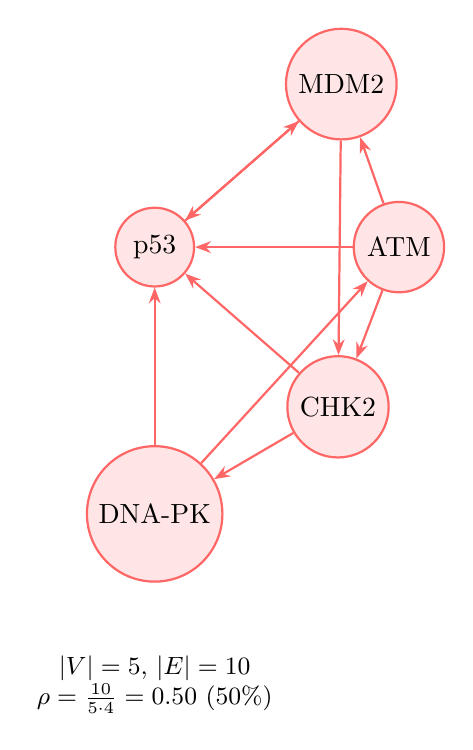
\begin{tikzpicture}[
		node distance=2cm,
		protein/.style={circle, draw=red!60, fill=red!10, thick, minimum size=1cm},
		interaction/.style={-{Stealth[length=2mm]}, thick, draw=red!60}
		]
		% Knoten (zentraler Hub)
		\node[protein] (p53) {p53};
		\node[protein, above right=1.2cm and 1.5cm of p53] (mdm2) {MDM2};
		\node[protein, right=of p53] (atm) {ATM};
		\node[protein, below right=1.2cm and 1.5cm of p53] (chk2) {CHK2};
		\node[protein, below=of p53] (dnapk) {DNA-PK};
		
		% Viele bidirektionale Interaktionen (hohe Dichte)
		\draw[interaction] (p53) -- (mdm2);
		\draw[interaction] (mdm2) -- (p53);
		\draw[interaction] (atm) -- (p53);
		\draw[interaction] (atm) -- (mdm2);
		\draw[interaction] (atm) -- (chk2);
		\draw[interaction] (chk2) -- (p53);
		\draw[interaction] (dnapk) -- (atm);
		\draw[interaction] (dnapk) -- (p53);
		\draw[interaction] (mdm2) -- (chk2);
		\draw[interaction] (chk2) -- (dnapk);
		
		% Dichte-Berechnung
		\node[below=0.8cm of dnapk, align=center, font=\small] {
			$|V| = 5$, $|E| = 10$ \\
			$\rho = \frac{10}{5 \cdot 4} = 0.50$ (50\%)
		};
	\end{tikzpicture}
\end{document}